The "Hand-Eye calibration (Robotics)" calibration method is used to determine the
reference between Tool Coordinate System (TCP) and Camera coordinate system
(position and orientation) when the VISOR\textsuperscript{\textregistered} is attached to the gripper.
\cite[page 102]{visor_user_manual}

The calibration process is automated within the robot program
such that operator could request to re-calibrate the camera w.r.t
robot TCP from the touch panel. The robot finishes the current
bending operation and then in next cycle, start with the auto-calibration.

% To include an image:
\begin{figure}[h]
    \centering
    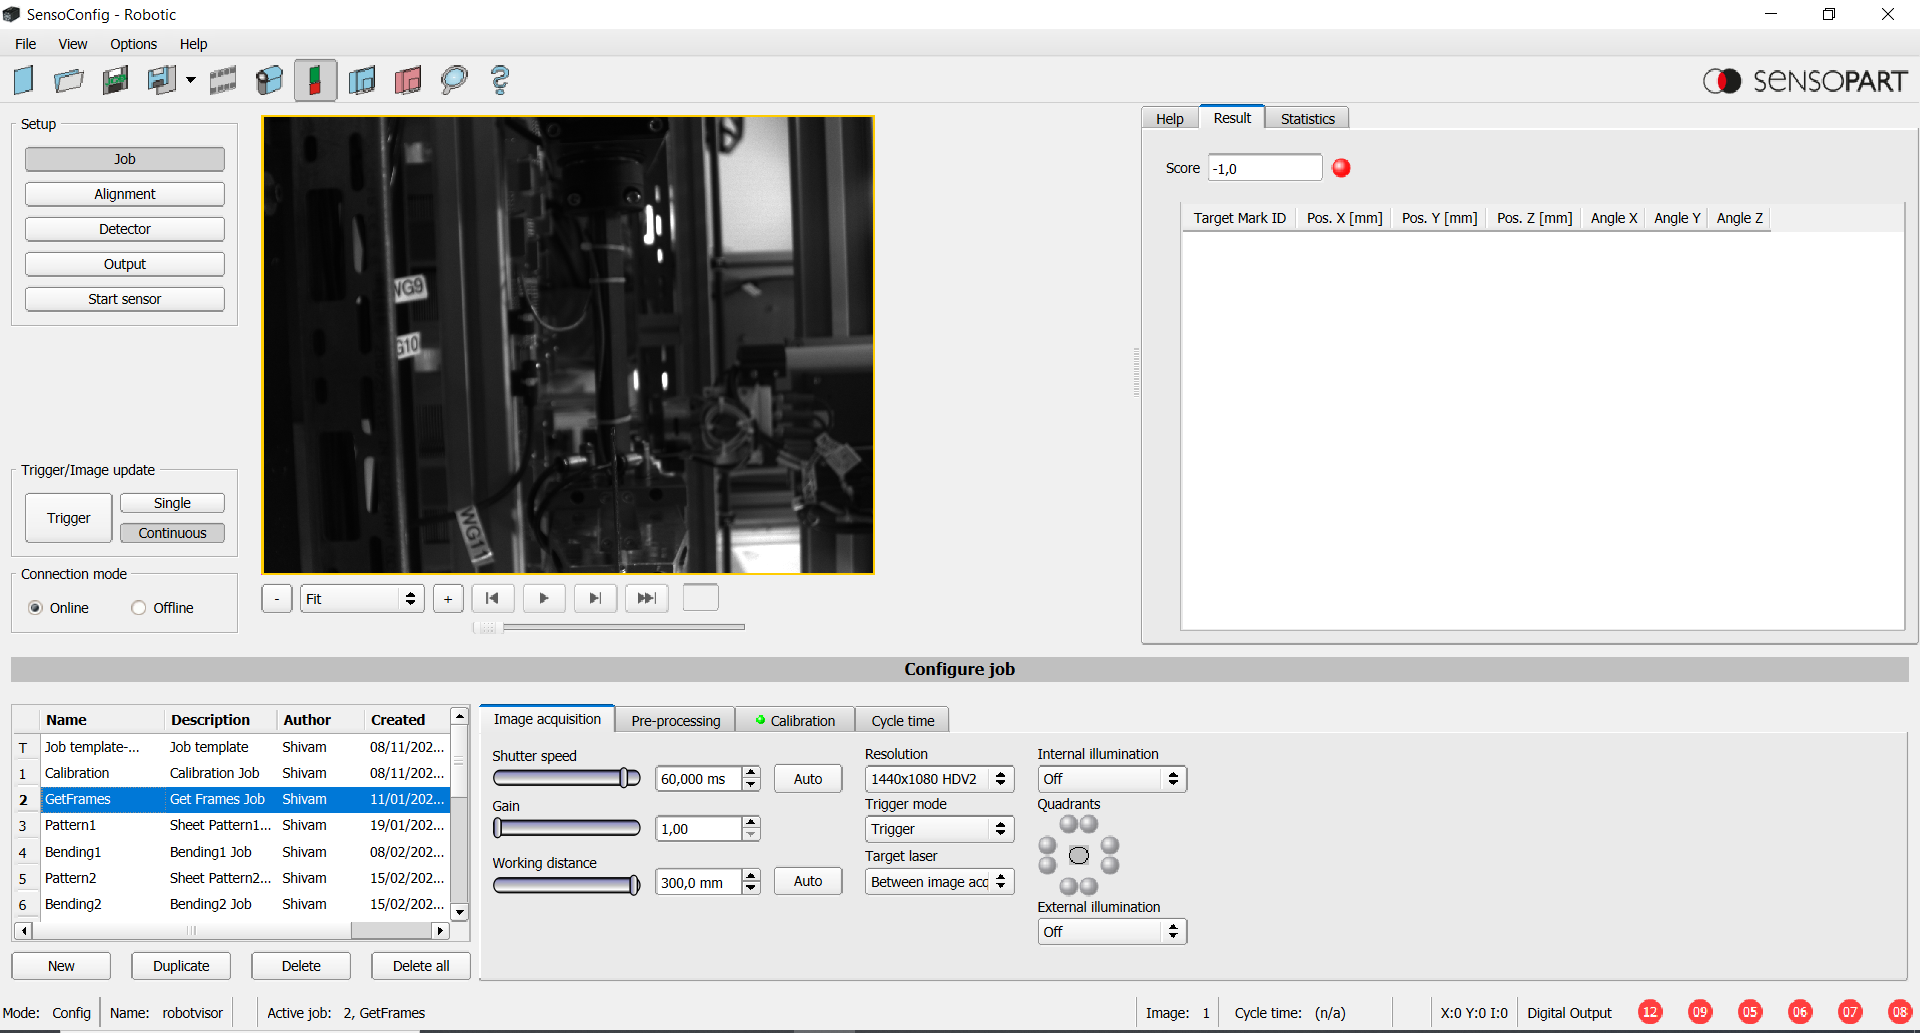
\includegraphics[width=\textwidth]{6. System Integration and Testing/6.2 Calibration Procedures/shutter_speed.PNG}
    \caption{A working distance of 300mm is set for the robotic camera}
    \label{fig:working-distance}
\end{figure}

\begin{figure}[h]
    \centering
    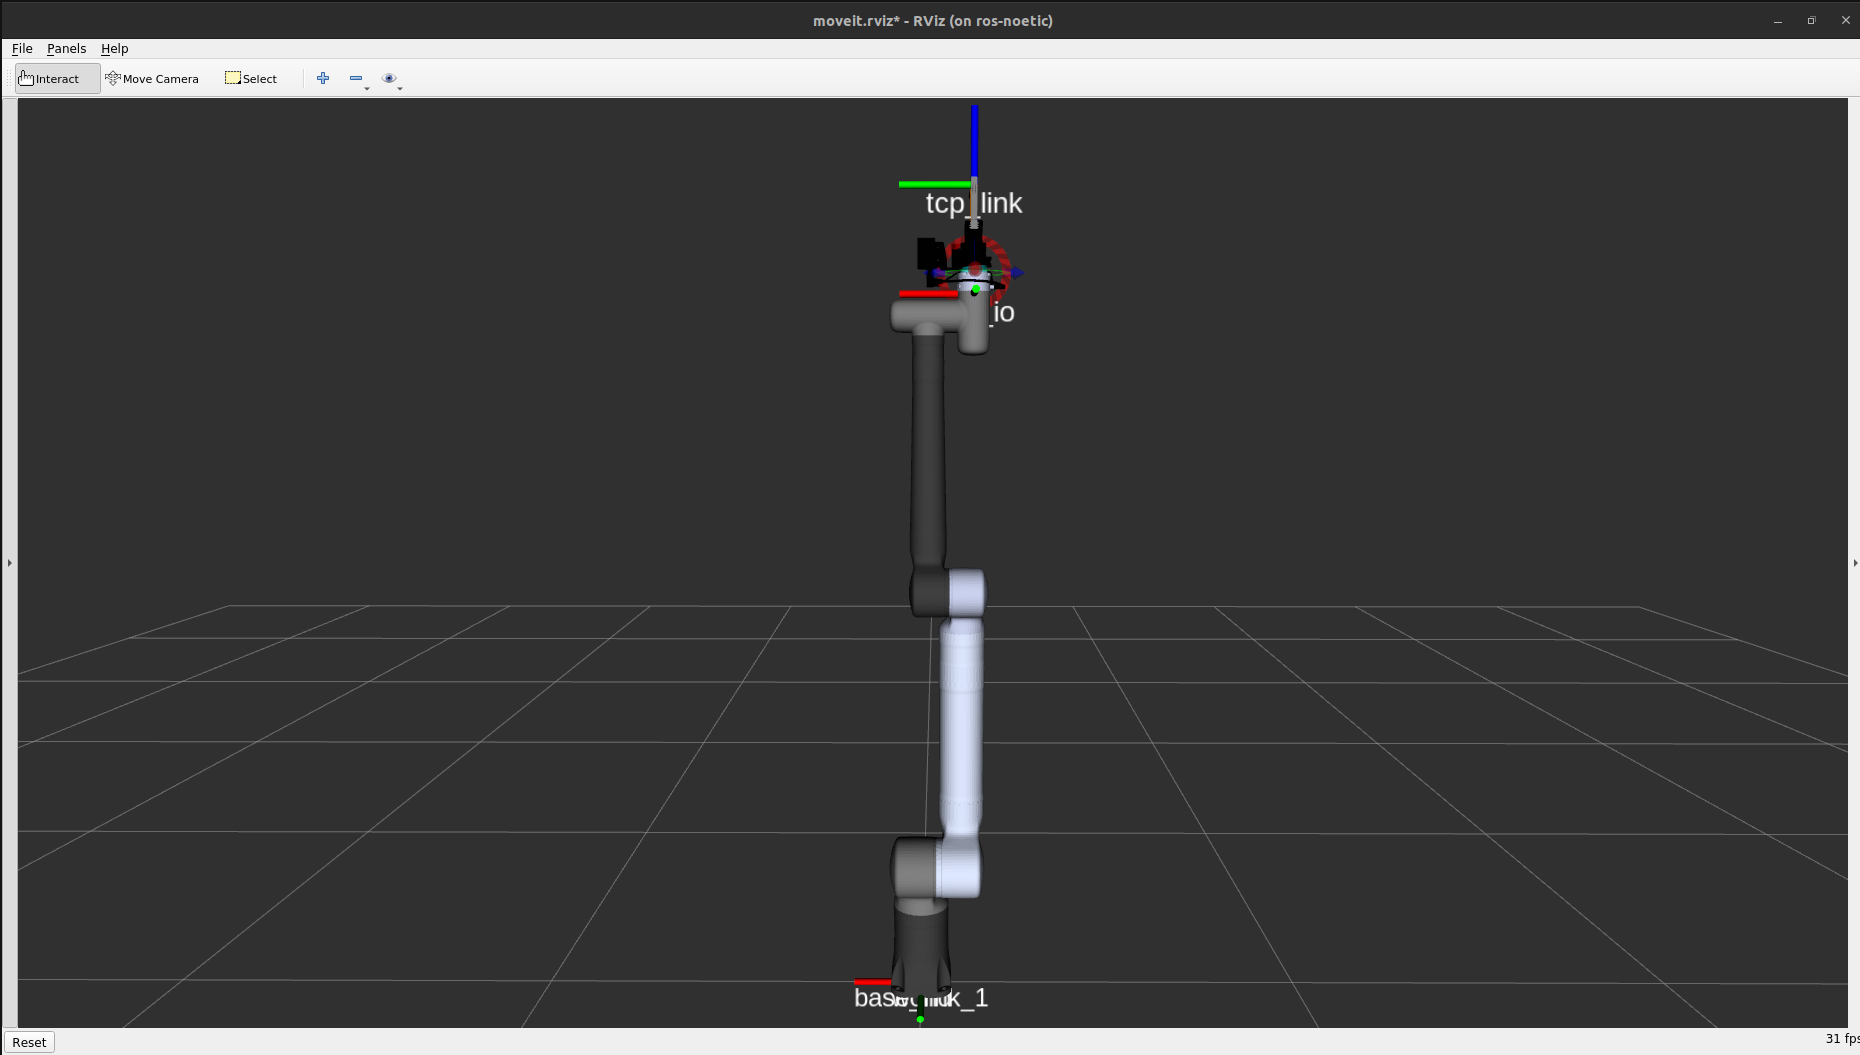
\includegraphics[width=\textwidth]{6. System Integration and Testing/6.2 Calibration Procedures/tcp.PNG}
    \caption{TCP is set at the end of gripper at a distance of 216mm from robot TOOL-IO}
    \label{fig:tcp}
\end{figure}


Calibration is a crucial procedure in the development of 
an automated robotic workcell, ensuring that all components
operate accurately and in harmony.
.\subsection{Robot Calibration}
Robot calibration ensures that the Kassow robot can accurately position its end effector for loading, bending, and unloading metal sheets. This involves:

\begin{itemize}
    \item \textbf{Kinematic Calibration}: Adjusting the robot’s kinematic model to correct any discrepancies between the theoretical model and the actual hardware. This includes measuring and compensating for joint offsets, link lengths, and joint angles.
    \item \textbf{Tool Center Point (TCP) Calibration}: Determining the exact position of the end effector or tool relative to the robot’s last joint. This is crucial for precise manipulation of metal sheets.
    \item \textbf{Workspace Calibration}: Defining the robot’s operational workspace and ensuring that all tasks are performed within this defined area, avoiding collisions and ensuring smooth operation.
\end{itemize}

\subsection{Camera Calibration}
Camera calibration is essential for the accurate detection of metal sheets and measurement of bending angles. The process involves:

\begin{itemize}
    \item \textbf{Intrinsic Calibration}: Determining the camera's internal parameters, such as focal length, optical center, and lens distortion. This is typically achieved using a calibration target (e.g., a checkerboard pattern) and specialized software tools.
    \item \textbf{Extrinsic Calibration}: Establishing the camera’s position and orientation relative to the robot or the workcell. This involves aligning the camera’s coordinate system with the robot’s coordinate system to ensure accurate detection and measurement.
    \item \textbf{Stereo Calibration (if applicable)}: If using a stereo camera setup for 3D perception, calibrating the relative position and orientation between the two cameras to obtain accurate depth information.
\end{itemize}

\subsection{Sensor Calibration}
Other sensors integrated into the workcell, such as force/torque sensors or additional proximity sensors, also require calibration to ensure accurate measurements and reliable operation. This involves:

\begin{itemize}
    \item \textbf{Zeroing Sensors}: Establishing a baseline or zero point for sensors to eliminate any offsets or biases in their readings.
    \item \textbf{Range Calibration}: Ensuring that sensors can accurately measure across their entire operational range, providing reliable data for the control system.
\end{itemize}

\subsection{Calibration Procedures}
The calibration process involves several systematic steps:

\begin{enumerate}
    \item \textbf{Setup Calibration Targets}: Place calibration targets within the robot’s workspace and at specific positions that the cameras will observe.
    \item \textbf{Data Collection}: Use the robot and cameras to collect data from the calibration targets. This includes moving the robot through its range of motion and capturing images from different angles.
    \item \textbf{Parameter Estimation}: Use calibration software to estimate the parameters of the robot’s kinematic model, the intrinsic and extrinsic parameters of the cameras, and the characteristics of any other sensors.
    \item \textbf{Validation}: Verify the calibration by performing tasks that require high precision and checking the accuracy of the results. Adjust calibration parameters as needed based on validation results.
    \item \textbf{Documentation}: Record the calibration parameters and procedures for future reference and troubleshooting.
\end{enumerate}

